\documentclass[a4paper]{article}
\usepackage[utf8]{inputenc}
\usepackage[ngerman]{babel}
\usepackage{listings}
\usepackage{float}
\usepackage[dvipsnames]{xcolor}
\usepackage{geometry}
\usepackage{color,graphicx,overpic}
\usepackage{amsmath,amsthm,amsfonts,amssymb}
\usepackage{tabularx}
\usepackage[many]{tcolorbox}
\usepackage{multicol}
\usepackage{mdwlist} %less space for lists

\newtheorem{definition}{Definition}
\newtheorem{proposition}{Proposition}
\newtheorem{beweis}{Beweis}

\pdfinfo{
  /Title (Betriebssysteme - Übung)
  /Creator (TeX)
  /Producer (pdfTeX 1.40.0)
  /Author (Studenten TU Ilmenau)
  /Subject ()
}

% Don't print section numbers
\setcounter{secnumdepth}{0}

%My Environments
\newtheorem{example}[section]{Example}


\newtcolorbox{myboxii}[1][]{
 breakable,
 freelance,
 title=#1,
 colback=white,
 colbacktitle=white,
 coltitle=black,
 fonttitle=\bfseries,
 bottomrule=0pt,
 boxrule=0pt,
 colframe=white,
 overlay unbroken and first={
 \draw[red!75!black,line width=3pt]
  ([xshift=5pt]frame.north west) -- 
  (frame.north west) -- 
  (frame.south west);
 \draw[red!75!black,line width=3pt]
  ([xshift=-5pt]frame.north east) -- 
  (frame.north east) -- 
  (frame.south east);
 },
 overlay unbroken app={
 \draw[red!75!black,line width=3pt,line cap=rect]
  (frame.south west) -- 
  ([xshift=5pt]frame.south west);
 \draw[red!75!black,line width=3pt,line cap=rect]
  (frame.south east) -- 
  ([xshift=-5pt]frame.south east);
 },
 overlay middle and last={
 \draw[red!75!black,line width=3pt]
  (frame.north west) -- 
  (frame.south west);
 \draw[red!75!black,line width=3pt]
  (frame.north east) -- 
  (frame.south east);
 },
 overlay last app={
 \draw[red!75!black,line width=3pt,line cap=rect]
  (frame.south west) --
  ([xshift=5pt]frame.south west);
 \draw[red!75!black,line width=3pt,line cap=rect]
  (frame.south east) --
  ([xshift=-5pt]frame.south east);
 },
}

\lstset{
	literate={ö}{{\"o}}1
	{ä}{{\"a}}1
	{ü}{{\"u}}1
}

\begin{document}
\begin{myboxii}[Disclaimer]
    Die Übungen die hier gezeigt werden stammen aus der Vorlesung \textit{Betriebssysteme}! Für die Richtigkeit der Lösungen wird keine Gewähr gegeben.
\end{myboxii}


%%%%%%%%%%%%%%%%%%%%%%%%%%%%%%%%%%%%%%%%%%%%%%%%%%%%%%%%%%%%%%%%%%%%%%%%%%%%%%%%%%%%%%%%%%%%%%%%%%%%%%%%%%%%%%%%%%%%
\section{Übung 1}
%##########################################
\subsection{Aufgabe 1}
\textit{Wie würden Sie heute, zu Beginn des Kurses, den Begriff "Betriebssystem" beschreiben? Sehen Sie Analogien zwischen den Aufgaben und Funktionen von Betriebssystemen und denen gesellschaftlicher oder wirtschaftlicher Einrichtungen?}
\vspace{10mm}

Begriff "Betriebssysteme" beschreiben: Verknüpfung zwischen Hard- und Software.
\begin{itemize*}
    \item Ermöglicht Kommunikation
    \item Software: Browser, Office, Bibiliotheken,...
    \item Betriebssystem: Betriebssystemdienste, Resourcenmanagement, Schnittstellen, Bibiliotheken,...
    \item Hardware: CPU, GPU, E/A, Speicher, Netzwerk,...
\end{itemize*}
eine Abstraktion von Hardware-Ressourcen, Sammlung von programmen,
Vorteil: Komplexität verborgen vor dem Nutzer

%##########################################
\subsection{Aufgabe 2}
\textit{Wie sind diejenigen Betriebssysteme in Erscheinung getreten, mit denen Sie bisher schon gearbeitet haben? Welche Aufgaben haben sie gelöst? Welche Probleme haben sie gezeigt?}
\vspace{10mm}
verschiedene Betriebssysteme:
\begin{itemize*}
    \item Universalsysteme (Windows, Linux, Mac, Android, iOS): Benutzerfreundlich, keine Spezialisierung (GUI gehört nicht dazu)
    \item eingebettete Systeme (Microkontroller): resourcensparend, belastbarkeit
    \item Echtzeitsysteme (motorsteuerung): deadlines!
    \item chipkarten/sicherheitssysteme: nicht wiederbeschreibbar, meist genau 1 Aufgabe
\end{itemize*}

%##########################################
\subsection{Aufgabe 3}
\textit{In der Vorlesung haben Sie ein breites Spektrum an Einsatzgebieten für Betriebssysteme kennen gelernt, das verdeutlichen sollte, welche sehr unterschiedlichen Anforderungen heute an Betriebssysteme gestellt werden. Kennen Sie über diese Szenarien hinaus Beispiele für Einsatzgebiete, in denen folgende eine zentrale Rolle spielen? Was wären die jeweiligen Konsequenzen, wenn ein Betriebssystem dabei diese Eigenschaften nicht besitzen würde?}
\vspace{10mm}
\begin{description*}
    \item[Echtzeitfähigkeit] einhalten von Fristen ist Hauptziel, harte oder weiche EZS
    \item[Robustheit] betrieb in widrigen Umgebungen (Umwelteinflüsse, Anwenderfehler)
    \item[Sicherheit] Security: schutz gegen Angriffe von außen (Verschlüsselung etc); Safety: Schutz gegen "Angriffe von innen" (Speichersicherheit etc)
    \item[Korrektheit] (gegenüber einer Spezifikation) Testen (keine vollständige Sicherheit), Verifikation (mathematischer Beweis)
    \item[Performanz] Geschwindigkeit von Anwenderprogrammen, Effiziente Algorithmen für BS Dienste
    \item[Sparsamkeit] BS Größe, energie- und ressourcenschonend
    \item[Skalierbarkeit] Lastskalierbarkeit (Bsp Online shops), Ressourcenskalierbarkeit
\end{description*}


%##########################################
\subsection{Aufgabe 4}
\textit{Wenn Sie auf einem der heute üblichen Computer Bürosoftware, Internetprogramme (Webbrowser, E-Mail-Clients etc.) und Audio/Video-Applikationen nutzen möchten und die Wahl eines Betriebssystems hätten: Welche der oben genannten und welche weiteren Eigenschaften würden Sie von diesem Betriebssystem erwarten?}
\vspace{10mm}
Anforderungen an Office-PC-BS (universalsystem): Interaktivität, Performance, Robustheit, korrektheit, sicherheit, sparsamkeit, bequemlichkeit, hohe abstraktionsebene


%##########################################
\subsection{Aufgabe 5}
\textit{Warum könnte es problematisch sein, ein und dasselbe Betriebssystem auf Großrechnern (Mainframes) und gleichzeitig auf eingebetteten Systemen einzusetzen?}
\vspace{10mm}
gleiches Betriebssystem für Großrechner und eingebetteten Systemen? Portierbarkeitsprobleme
\begin{itemize*}
    \item Aufgaben sehr unterschiedlich; Batch-Verarbeitung, Interaktiv
    \item Ressourcen Verwaltung/Größen
    \item Platformspezifische Einheiten (Befehlssätze, RISC vs CISC)
    \item Funktionsumfang
\end{itemize*}

%##########################################
\subsection{Aufgabe 6}
\textit{Welche Vorteile hat es aus Anwendersicht, Betriebssysteme als Virtualisierung von Maschinen zu verstehen?}
\vspace{10mm}
Vorteile für Anwender die Betriebssysteme als Virtualisierung zu sehen
\begin{itemize*}
    \item Bequemlichkeit
    \item Beherschbarkeit + Isolation
\end{itemize*}

\newpage
%%%%%%%%%%%%%%%%%%%%%%%%%%%%%%%%%%%%%%%%%%%%%%%%%%%%%%%%%%%%%%%%%%%%%%%%%%%%%%%%%%%%%%%%%%%%%%%%%%%%%%%%%%%%%%%%%%%%
\section{Übung 2}
%##########################################
\subsection{Repetitorium}
\begin{itemize*}
    \item \textbf{Welcher Zusammenhang besteht zwischen den Konzepten Nebenläufigkeit und Parallelität? Wann können Aktivitäten auf einem System nur pseudoparallel ausgeführt werden?} Nebenläufigkeit ist die Voraussetzung für Parallelität. Nebenläufigkeit beschreibt wiederum den Umstand, dass zwischen zwei Aktivitäten keine kausalen Abhängigkeiten bestehen. Parallel, wenn zwei oder mehr Aktivitäten zeitgleich/ zeitlich überlappend ausgeführt werden können. Das wiederum bedeutet, dass man Aufgaben, bei welchen die Teillösungen immer aufeinander aufbauen nicht parallelisieren kann. Allerdings ist die gleichzeitige Berechnung von unabhängigen Lösungen kein Problem und somit kann sich auch ein enormer Geschwindigkeitszuwachs bieten. Aktivitäten können nur dann echt parallel ausgeführt werden, wenn auch mehrere unabhängige Prozessorcores dafür zur Verfügung stehen, das bedeutet, sobald nicht mehrere Prozessoren verfügbar sind, kann die Parallelität nur durch zeitliches Switching simuliert werden. Pseudoparallel weiter bei Abhängikeit (z.b. Synchronisation)
    \item \textbf{Wozu dienen Prozessmodelle? Aus welchen Bausteinen setzt sich ein Prozessmodell zusammen? Welche finden sich typischerweise in Prozessdeskriptoren wieder?} Da wir einem Computer nicht einfach mehrere Aufgaben ohne Kontext und ähnliches vorwerfen können und das Rechnen darauf beginnen können, müssen wir etwas neues Einführen. Hier wählen wir Prozesse. Prozesse sind eine Betriebssystemabstraktion zur vollständigen Beschreibung einer sequentiell ablaufenden Aktivität. Im weiteren Verlauf ist es nun so, dass parallele Aufgaben durch parallele Prozesse beschrieben/repräsentiert werden. \\
    Ein Prozessmodell definiert nun Prozesse und die konkreten Prozesseigenschaften: zum Beispiel: Semantik der Operationen auf Prozessen, also die Auswirkungen von Erzeugen, Beenden, Anhalten, Fortsetzen, sowie auch die nichtfunktionalen Eigenschaften von Prozessen, wie beispielsweise die Echtzeiteigenschaften, Safetyeigenschaften, Securityeigenschaften.\\
    Ein Prozessdeskriptor oder PCB „Process Control Block“ beinhaltet Informationen zur Identifikation, Größe, Position, Zugriffsberechtigungen und Verwendung eines Segments und erlaubt somit erst das parallele Rechnen.\\
    Aufbau des Prozessmodells/ Process Control Block: Identifikationsbereicht + Schedulinginformation + Programmkontext (Instruction Pointer + Stackpointer + PSR) + Ereignismanagement + Accounting + Rechte + Ressourcen
    \item \textbf{Aus welchem Grund wurde das Thread-Konzept entwickelt? Welche zwei eigentlich unabhängigen Konzepte sind im Modell des ursprünglichen (Schwergewichts-)Prozesses vereint?} Das Thread-Modell wurde für die Parallelisierung nebenläufiger Aktivitäten erschaffen, da sich zeigte, dass ein neuer Prozess pro nebenläufiger Aufgabe eher unpraktisch ist. Die Hauptprobleme oder die wichtigsten negativen Aspekte zeigten sich bei dem hohen Managementaufwand, den hohen Kosten für die Isolation und die hohen Kosten für die Kommunikation der Prozesse untereinander. \\
    Im ursprünglichen schwergewichtigen Prozessen war das Konzept des Ressourcenmanagements und das Management der Parallelität vereint.
    \item \textbf{Wozu dienen Prozess- bzw. Threadzustände? Welche elementaren Zustände finden sich in jedem Prozessmodell?} Thread und Prozesszustände erlauben es mehrere Threads (pesudo)parallel auszuführen, bzw. erlauben das Scheduling, indem man per Zustand bestimmt, was ein Thread gerade macht. Hier gibt es als unterschiedliche Zustände „frisch“, „aktiv“, „blockiert“, „beendet“, „bereit“.
    \item \textbf{Warum benötigt jeder Thread einen eigenen Stack?} Da jeder Thread seine eigene Ausführungssequenz / seinen eigenen Code haben kann, muss er einen eigenen Stack (LIFO Speicher) haben, auf den er den Inhalt seines Programmzählers schieben/einfügen kann (wenn z.B. Funktionsaufrufe und Rückgaben stattfinden).
    \item \textbf{Worin besteht der Unterschied zwischen Kernel- und User-Level-Threads? Welche Vor- und Nachteile besitzt die jeweilige Form? Wo befinden sich die PCB- und TCB-Datenstrukturen?} Kernel-Level-Threads werden direkt durch das OS verwaltet und das Thread Management geschieht direkt durch den Kernel. Dadurch, dass sowohl die Kontextinformation als auch die Prozessthreads alle durch den Kernel gemenaged werden, kann man sagen, dass Kernel-level-threads typischerweise eher langsamer als User-Level-Threads sind und ihre Performanz durch Parallelität erreichen. (Multithreadingbetriebssystem)\\
    \begin{itemize*}
        \item Vorteile: Effiziente Nutzung von Multicore-Architekturen. Mehrere Threads des selben Prozess können auf verschiedenen Prozessoren geschedult werden. Ein blockierender Systemaufruf in einem Thread blockiert nicht auch gleichzeitig alle anderen Threads des gleichen Prozess.
        \item Nachteile: Da der Kernel sowohl Threads als auch Prozesse verwalten und planen muss, benötigt er einen vollständigen Thread-Kontrollblock (TCB) für jeden Thread, um Informationen über Threads zu erhalten. Dies führt zu einem erheblichen Overhead und erhöht die Komplexität des Kernels. Die Threads auf Kernel-Ebene sind langsam und ineffizient. Beispielsweise sind die Thread-Operationen hundertmal langsamer als die Threads auf Benutzerebene.
        \item User Level Threads werden durch Nutzer implementiert und der Kernel selbst hat kein Wissen über die Existenz dieser Threads und behandelt diese, als wären sie Single-Thread Prozesse. Userlevelthreads sind kleiner und schneller als kernel level threads. Sie werden durch einen Programmzähler (PC), Stapel, Register und einen kleinen Prozess-Steuerblock dargestellt. Außerdem gibt es keine Kernel-Beteiligung an der Synchronisation für Threads auf Benutzerebene.
        \item ULT: Thread-Implementierung in Anwendung (OS kennt keine Threads)\\
        Vorteile:\\
        Threads auf Benutzerebene sind einfacher und schneller zu erstellen als Threads auf Kernel-Ebene. Sie lassen sich auch leichter verwalten.
        Threads auf Benutzerebene können auf jedem Betriebssystem ausgeführt werden.
        In Threads auf Benutzerebene sind keine Kernelmodus-Privilegien zum Threadwechsel erforderlich.
        Thread-Management ohne Systemaufrufe
        anwendungsindividuelle Thread-Schedulingstrategien möglich (für Spezialanwendungen sinnvoll)\\
        Nachteile: \\
        Multithread-Anwendungen in Threads auf Benutzerebene können Multiprocessing nicht zu ihrem Vorteil nutzen.
        Der gesamte Prozess wird blockiert, wenn ein Thread auf Benutzerebene blockierende Operationen durchführt.\\
        Beim Kernel-level-Thread befinden sich sowohl der PCB als auch TCB im Kernelspace. Beim User-level-Thread befinden sich PCB im Kernelspace und der TCB im Userlevel.
    \end{itemize*}
\end{itemize*}
%##########################################
\subsection{Aufgabe 1: Prozesserzeugung in Linux-Systemen}
\textit{In Betriebssystemen der Unix/Linux-Familie werden neue Prozesse durch den fork-Systemaufruf erzeugt. Dabei entsteht sukzessive eine Abstammungshierarchie, in der ein Prozess, der ein fork() (erfolgreich) ausführt, zum Elternprozess ("parent") des von ihm erzeugten Kind-Prozesses ("child") wird. Die bei Unix/Linux-Systemen benutzte Technik funktioniert wie folgt: Durch fork wird eine nahezu exakte Kopie des Elternprozesses zum Zeitpunkt des fork()-Aufrufs erzeugt, bei der der neue Kindprozess eine Vielzahl der Eigenschaften des Elternprozesses erbt. Falls der Kindprozess ein anderes als das vom Elternprozess vererbte Programm ausführen soll, kann das Kind unmittelbar nach fork einen Systemaufruf der exec[ute]-Familie verwenden, der das durch den aufrufenden Prozess ausgeführte Programm austauscht.}
\vspace{10mm}
\textit{a) Informieren Sie sich über $fork$ und $exec*$ und finden Sie Antworten auf die folgenden Fragen. Wie unterscheiden sich Eltern- und Kindprozess unmittelbar nach dem fork()-Aufruf?}

Unterscheidung: getrennte Speicherbereiche, unterschiedliche PIDs, Programmierung gleich
Direkt nach dem fork Aufruf unterscheiden sich Vater und Kindprozess durch:
\begin{itemize*}
    \item Das Kind hat seine eigene und einzigartige PID, also ProzessID
    \item Die ProzessID des Vaterprozesses des Kindes ist die selbe wie die ProzessID des Vaters.
    \item Das Kind erbt keine Speichersperren/Memorylocks der Eltern
    \item Prozessressourcenauslastung und CPU-Zeitzähler werden im Kind auf 0 gesetzt
    \item Der Satz ausstehender Signale ist ursprünglich leer
    \item Das Kind erbt keine Semaphoranpassungen des Elternteils
    \item Das Kind erbt keine prozessbezogenen Datensatzsperren von seinem Elterneteil
    \item Das Kind erbt keine Zeitgeber von seinem Elterneteil
    \item Das Kind erbt keine austehenden E/A Operationen oder Kontexte
\end{itemize*}
Weiterhin gibt es einige Linux-Spezifische Prozessattribute welche sich verändern, hierzu zählen insbesondere:
\begin{itemize}
    \item Das Kind erbt keine Verzeichnisänderungsbenachrichtigungen von seinem Elternteil
    \item Speicherzuordnungen, die mit dem $madvise(2)$ MADV\_DONTFORK-Flag markiert wurden, werden nicht über einen $Fork()$ vererbt.
\end{itemize}

\textit{Woran können sich Eltern- und Kindprozess unmittelbar nach einem fork()-Aufruf selbst erkennen ("Wer bin ich?")? Finden Sie mindestens 3 Möglichkeiten. }

Selbsterkkennung: $getpid()$, $getppid()$, $system()$-calls, Rückgabewert von $fork()$

\textit{Welche unterschiedlichen Werte kann der Funktionsaufruf fork() zurückgeben, und was bedeuten sie?}
\vspace{10mm}

Bei Erfolg wird im Elternprozess der PID des Kindprozesses >0 zurückgegeben, im Kindprozess wird 0 zurückgegeben. Bei einem Fehlschlag wird -1 im Elternprozess zurückgegeben, es wird kein Kindprozess erstellt und errno wird entsprechend gesetzt.

Rückgabewert von $fork()$:
\begin{itemize*}
    \item PID des Kindes von Parent
    \item 0 im Kindprozess
    \item -1 Fehler (errno gesetzt)
\end{itemize*}

\textit{b) Demonstrieren Sie mit dem einfachen C-Programm p1 (in der Anlage), dass nach der Ausführung von fork() tatsächlich zwei Prozesse existieren.}
\vspace{10mm}
$cc -o p1 p1.c$ // Kompiliert das Programm
Dann in selbem Directory ./p1, dies startet das Programm


\textit{c) Führen Sie Programm p2 aus. Dieses enthält einen execl-Systemaufruf, mit dem ein Programm p4 ausgeführt werden soll. Das Programm p4 muss dabei ein (mit dem C-Compiler) übersetztes, ausführbares Programm im gleichen Verzeichnis sein. Sie können dazu das vorgegebene Programm p4 verwenden, das lediglich einen Ausdruck erzeugt.}
\vspace{10mm}


\textit{d) Wie viele Prozesse werden durch das Programm p3 erzeugt? Warum? Was passiert, wenn execl() nicht erfolgreich ausgeführt werden kann, weil z. B. das Programm p4 nicht gefunden wird? Führen Sie zur Kontrolle p3 aus, während das Programm p4 einmal existiert und ein weiteres Mal, während dieses nicht existiert.}
\vspace{10mm}
Es werden insgesamt 4 Prozesse durch die Ausführung von p3 erzeugt.

Erklärung:
Es werden, falls es sich um einen Kindprozess handelt, fork() also = 0 ist, dessen PID und die des Elternknotens ausgegeben.
Weiterhin wird, falls es sich um einen Kindknoten handelt, das Kindprozessimage durch execl durch das Prozessimage p4 ersetzt.

Sollte es sich allerdings nicht um einen Kindknoten handeln, dann wird die PID des Elternprozess ausgegeben.

Dann wird unabhängig von der bisherigen Auswahl ein Fork erstellt, „PID terminating“ ausgegeben und wait(NULL) aufgerufen. wait(NULL) blockiert den Elternprozess, bis eines seiner Kinder beendet ist. Wenn der Kindprozess beendet wird, bevor der Elternprozess wait(NULL) erreicht, wird der Kindprozess zu einem Zombie-Prozess, solange bis der Elternprozess auf ihn wartet und ihn aus dem Speicher freigibt.

Im Fall, dass p4 nicht vorhanden ist, wird zuerst der Elternprozess ausgegeben. Dann wird ein Fork erstellt und Terminating ausgegeben. Der Elternprozess verfällt in den Wartemodus. Daraufhin wird p3 wieder aufgerufen, da es sich nun um einen Fork handelt, wird Ausgegeben, dass ein Kind erstellt wurde und es wird versucht dieses Kindimage durch das p4 image zu ersetzen. Dies funktioniert allerdings nicht, also wird von execl -1 zurückgegeben.



%##########################################
\subsection{Aufgabe 2: Prozessdeskriptoren und Prozesszustände}
\textit{Beschäftigen Sie sich mit dem Shell-Kommando $ps$. Es dient dazu, bestimmte Informationen aus den Prozessdeskriptoren ausgewählter Prozesse auszugeben. Die ausgewählte Prozessmenge und der Umfang der wiedergegebenen Informationen kann dabei durch entsprechende Parameter beeinflusst werden. So bedeutet z. B. $ps -el$, dass eine Liste mit vielen Parametern (l, "long") für alle Prozesse (e) erzeugt wird. Aus Gründen der Übersichtlichkeit kann auch $ps -al$ verwendet werden.}
\vspace{10mm}
\textit{a) Welche Prozesszustände sind in Linux-Betriebssystemen definiert, und wie erkennt man diese an den Ausgaben von ps?}
\vspace{10mm}
Man erkennt die Zustände an dem STAT Wert.

Mit ps lassen sich Daten über die Prozesse in der Prozeßtabelle anzeigen. Die Prozeßtabelle wird mit einer Titelzeile ausgegeben. Die Spalten haben folgende Bedeutung:
\begin{tabular}{c|c}
    PID     & Die Process-ID des Prozesses                                                                                                                                                                                                                                                                                                                                               \\
    PPID    & Die Parent Process ID des Prozesses                                                                                                                                                                                                                                                                                                                                        \\
    UID     & Die User ID des Users, dem der Prozeß gehört                                                                                                                                                                                                                                                                                                                               \\
    USER    & Der Username des Users, dem der Prozeß gehört                                                                                                                                                                                                                                                                                                                              \\
    PRI     & Die Priorität des Prozesses. Höhere Werte bedeuten höhere Priorität.                                                                                                                                                                                                                                                                                                       \\
    NI      & Der Nice-Wert des Prozesses. Höhere Werte bedeuten geringere Priorität.                                                                                                                                                                                                                                                                                                    \\
    SIZE    & Die Größe des Codes plus Daten plus Stack KiloByte                                                                                                                                                                                                                                                                                                                         \\
    TSIZE   & Die Größe des Codes in KiloByte. ELF Proz werden nicht korrekt dargestellt                                                                                                                                                                                                                                                                                                 \\
    DSIZE   & Die Größe der Daten und Stack in Kilobyte Prozesse werden nicht korrekt dargestellt                                                                                                                                                                                                                                                                                        \\
    TRS     & Text Resident Size - Die Größe des resident Code-Blocks in KiloByte                                                                                                                                                                                                                                                                                                        \\
    SWAP    & Größe des ausgelagerten Bereichs des Tasks                                                                                                                                                                                                                                                                                                                                 \\
    D       & Größe der als Dirty markierten Speicherseiten                                                                                                                                                                                                                                                                                                                              \\
    LIB     & Größe der Library-Speicherseiten - Funktion nicht bei ELF-Prozessen.                                                                                                                                                                                                                                                                                                       \\
    RSS     & Die Größe des physikalische Speichers, den das Programm benutzt. Für ELF-Format werden hier auch die Libraries mitgezählt, bei a.out Format nicht.                                                                                                                                                                                                                         \\
    SHARE   & Die Größe der benutzten Shared-Libraries des Prozesses.                                                                                                                                                                                                                                                                                                                    \\
    STAT    & Der Status des Prozesses. Das kann entweder ein S für schlafend, D für ununterbrechbar schlafend (dead), R für laufend (running) oder T für angehalten (traced). Dieser Angabe kann noch ein < für einen negativen Nice-Wert, ein N für einen positiven Nice-Wert oder ein W für einen ausgelagerten Prozeß folgen. (Das W funktioniert nicht richtig für Kernel-Prozesse) \\
    WCHAN   & Die Kernelfunktion, die der Task gerade nutzt.                                                                                                                                                                                                                                                                                                                             \\
    TIME    & Die gesamte CPU-Zeit, die der Prozeß verbraucht hat, seit er gestartet wurde.                                                                                                                                                                                                                                                                                              \\
    \%CPU   & Die CPU-Zeit, die der Prozeß seit dem letzten Bildschirm-Update verbraucht hat, dargestellt als Prozentsatz der gesamten CPU-Zeit.                                                                                                                                                                                                                                         \\
    \%MEM   & Der Anteil des Speichers, den der Task nutzt.                                                                                                                                                                                                                                                                                                                              \\
    COMMAND & Das Kommando, mit dem der Prozeß gestartet wurde.                                                                                                                                                                                                                                                                                                                          \\
    TTY     & Die Terminalleitung des Prozesses.                                                                                                                                                                                                                                                                                                                                         \\
\end{tabular}

\textit{b) Starten Sie das Programm p5, in dem der durch $fork()$ erzeugte Kindprozess in einer Endlosschleife läuft (Zweck?). Welche Prozesszustände haben Eltern- und Kindprozess? Beobachten Sie, welche Komponenten der Prozessdeskriptoren sich in Abhängigkeit von der Zeit ändern und interpretieren Sie dies.}
\vspace{10mm}
Das einzige was sich an Programm p5 zeigt, ist dass sich die Rechenzeit erhöht, sonst werden keine Prozesse mehr geforkt. Der Parentprozess ist in Zustand S+, d.h. er läuft zwar im Vordergrund, ist allerdings im unterbrechbaren Schlaf und wartet darauf, dass ein Event fertiggestellt wird. Der Kindprozess ist im Zustand R+, was bedeutet, dass er gerade ausgeführt wird und im Vordergrund läuft.

Im Lauf der Zeit verändert sich vor allem die Laufzeit des Programms, also die CPU Zeit


\textit{c) Wenn ein Prozess auf ein sogenanntes Ereignis warten muss, beispielsweise eine Eingabe, dann ändert sich dessen Zustand. Starten Sie Programm p6, welches mittels $getchar()$ auf eine Eingabe vom Standardeingabegerät (ohne weitere Maßnahmen ist dies die Tastatur) wartet, und untersuchen Sie die Zustandsinformationen des wartenden Prozesses.}
\vspace{10mm}
Der Prozess p6 selbst ist im S+ State, was bedeutet, dass er im aufweckbaren Zustand ist und auf die Eingabe wartet. Die CPU Zeit ändert sich nicht, was bedeutet, dass keine Zeit verbraucht wird.

\textit{d) Mit dem Systemaufruf $sleep()$ kann sich ein Prozess selbst "schlafen legen". Starten Sie p7 und untersuchen Sie, welchen Zustand der hierdurch erzeugte Prozess nach dem Aufruf von $sleep()$ einnimmt.}
\vspace{10mm}
Bei aufruf von sleep() wird der Prozess sofort alle CPU Ressourcen freigeben, also fällt die CPU Auslastung für den Prozess auf 0, weiterhin wird der Zustand für die Zeit von sleep(time) auf S+ gesetzt, nach Ablauf der Zeit wird es sich wieder auf R+ (also runnable) wechseln. CPU Zeit wird währenddessen natürlich auch nicht verbraucht.

%##########################################
\subsection{Aufgabe 3: Dateiformate ausführbarer Programme}
\textit{Kompilierte Programme liegen immer in einem genau definierten Format vor. Ziel dieser Aufgabe ist es, Erkenntnisse darüber zu gewinnen, wie ein Betriebssystem aus einem kompilierten Programm einen Prozess erzeugt. Ein in Linux-Betriebssystemen verbreitetes Binärformat ist ELF (Executable and Link Format), welches Gegenstand dieser Aufgabe ist.}
\vspace{10mm}
\textit{a) Im Mittelpunkt Ihrer Recherchen über ELF sollte stehen, welche Informationen das Betriebssystem zur Erzeugung eines Prozesses benötigt und wo und wie diese in ELF zu finden sind. Berücksichtigen Sie ebenfalls die Metainformationen, die sich im ELF-Header befinden. Finden Sie Antworten auf die folgenden Fragen.
    \begin{itemize}
        \item \textbf{Wie findet man (bzw. das Betriebssystem) die erste auszuführende Instruktion innerhalb des Text-Segments?} Erste Instruktion $e\_entry$ gibt die virtuelle Adresse an, an welcher der Prozess zuerst beginnt.
        \item \textbf{Auf welche Weise bekommen bereits im Quellprogramm (z. B. C-Programm) initialisierte Variablen ihre Anfangswerte vor dem Start der Ausführung eines Programmes?} Die Initialisierung mit Anfangswerten findet durch Einträge im Programmimage statt. Hier gibt es die Sections .data und .data1, welche beide jeweils Informationen zur Inititalisierung beinhalten.
        \item \textbf{Woran erkennt man, um welchen Typ einer in ELF dargestellten Datei es sich handelt? Für welche Dateitypen ist ELF prinzipiell vorgesehen?} Man erkennt dies an dem Eintrag in $e\_type$ im ELF Header (NoFileType, Relocatable, Executable, Shared Object, CoreFile, ProcessorSpecific)
        \item \textbf{Unterscheiden sich ELF-Dateien für 32-Bit- und 64-Bit-Prozessorarchitekturen? Woran ist das gegebenenfalls erkennbar?} $e\_ident/EI$-CLASS identifiziert die Kapazität oder die Dateiklasse. Falls der Wert auf 1 ist, so handelt es sich um 32 Bit Objekte, falls der Wert auf 2 gesetzt ist um 64 Bit Werte
        \item \textbf{Welchen Zweck haben die so genannten Sektionen (sections) bzw. die program headers?} Die Headertabelle einer Objektdatei ermöglicht es, alle Abschnitte der Datei zu finden. Die Headertabelle ist ein Array von $Elf32\_Shdr$-Strukturen. Ein Tabellenindex der Headertabelle ist ein Subskript in diesem Array. Das $e\_shoff$-Mitglied des ELF-Headers gibt den Byte-Offset vom Anfang der Datei in die Sectionheadertable; $e\_shnum$ gibt an, wie viele Einträge die Sektionskopftabelle enthält; $e\_shentsize$ gibt die Größe jedes Eintrags in Bytes an. Die Programmkopftabelle einer ausführbaren oder gemeinsam genutzten Objektdatei ist eine Anordnung von Strukturen, die jeweils ein Segment oder andere Informationen beschreiben, die das System benötigt, um das Programm für die Ausführung vorzubereiten. Ein Objektdateisegment enthält einen oder mehrere Abschnitte. Programm-Header sind nur für ausführbare und gemeinsam genutzte Objektdateien von Bedeutung. Eine Datei-Spezifikation bestimmt seine eigene Programm-Header-Größe mit der $e\_phentsize$ des ELF-Headers und $e\_phnum$-Mitglieder. Der ELF-Programmheader wird durch den Typ $Elf32\_Phdr$ oder $Elf64\_Phdr$ je nach Architektur gegeben.
        \item \textbf{Welche Bedeutung hat eine Symboltabelle als Teil einer in ELF dargestellten Datei?} Die Symboltabelle einer Objektdatei enthält Informationen, die benötigt werden, um die symbolischen Definitionen und Verweise eines Programms zu lokalisieren und zu verschieben. Ein Symboltabellenindex ist ein Subskript in diesem Array. Index 0 bezeichnet sowohl den ersten Eintrag in der Tabelle als auch den undefinierten Symbolindex.
    \end{itemize}}
\vspace{10mm}

\textit{b) Untersuchen Sie experimentell Binärdateien hinsichtlich ihrer ELF-Metainformationen. Hierzu können Sie die Werkzeuge readelf und objdump verwenden, um zu ermitteln, welche konkreten Informationen eine Datei im ELF-Format enthalten kann. Als Beispiele sollen mindestens die folgenden ELF-Binärdateien dienen:
    \begin{itemize}
        \item das ls-Utility, zu finden im Verzeichnis /bin,
        \item die Executable zum Programm p1.c (siehe Anlage zu Aufgabe 1),
        \item eine dynamisch ladbare Bibliothek aus dem Verzeichnis /lib oder /usr/lib.
    \end{itemize}}
\vspace{10mm}
\begin{lstlisting}
    readelf -a p1
\end{lstlisting}

\newpage
%%%%%%%%%%%%%%%%%%%%%%%%%%%%%%%%%%%%%%%%%%%%%%%%%%%%%%%%%%%%%%%%%%%%%%%%%%%%%%%%%%%%%%%%%%%%%%%%%%%%%%%%%%%%%%%%%%%%
\section{Übung 3}
%##########################################
\subsection{Repetitorium}
\begin{itemize*}
    \item \textbf{Durch welche Ereignisse wechselt ein Thread vom Zustand aktiv in den Zustand blockiert? Durch welche in den Zustand suspendiert?}
    \begin{itemize}
        \item Der Zustandswechsel geschieht beispielsweise dadurch, dass ein aktiver Prozess auf E/A Operationen oder Timer warten muss, aufgrund dessen wird er dann in den Zustand blockiert geschickt, weiterhin kann es an einem Mangel an Betriebsmitteln liegen.
        \item Ein Prozess wechselt in den Zustand suspendiert/ready, wenn es initial rechenbereit war, allerdings aus dem Hauptspeicher geswapped wurde und auf einem externen Speicher ausgelagert ("swapping") wurde. Der Prozess wird wieder aktiv, wenn er aus dem externen Speicher zurück in den Hauptspeicher geswappt wird.
        \item Ein Prozess wechselt in den Zustand suspendiert/blockiert. Vom Konzpet ähnlich dem des Suspendiert/ready, mit dem Unterschied, dass der Prozess eine E/A Operation ausführte oder darauf wartete und ein Mangel an Hauptspeicher für die Auslagerung sorgte. Sobald allerdings die E/A Operation abgeschlossen ist, kann er in den Zustand suspendiert/bereit wechseln.
        \item Der Nutzer kann selbst suspenderieren, allerdings geschieht es typischerweise eher durch das OS selbst. (z.b. durch Überlastungssituation)
    \end{itemize}
    \item \textbf{Welche Auswirkung hat im Round-Robin-Schedulingalgorithmus die Veränderung der Größe der Zeitscheibe?}
    \begin{itemize}
        \item Sollte eine große Zeitscheibe eingesetzt werden, so gibt es wenige Threadwechsel, dadurch einen geringen Schedulingoverhead, allerdings ist die Reaktivität eher schlecht, zudem entstehen bei nicht-preemptiver Implementierung viele Abschnitte mit Leerlaufsituationen.
        \item Sollte eine kleine Zeitscheibe verwendet werden so hat man zwar einen sehr großen Overhead durch ständige Threadwechsel, allerdings eine sehr hohe Reaktivität.
        \item In der Praxis sind typische Zeitscheiben zwischen 20-50ms lang.
    \end{itemize}
    \item \textbf{Round-Robin-Scheduler verwalten normalerweise eine oder mehrere Listen von Prozessen, wobei jeder lauffähige Prozess genau einmal aufgeführt wird. Was würde passieren, wenn ein Prozess 2x in einer Liste stehen würde? Aus welchen Gründen könnte man so etwas erlauben?}
    \begin{itemize}
        \item Wenn ein Prozess häufiger in der Liste stehen würde, so würde dieser anteilig gesehen häufiger zur Ausführung zugelassen werden, was also einer Erhöhung der Priorität gleich kommen würde, allerdings kommt er dadurch nicht unbedingt schneller zur Ausführung. Falls er n-mal in der Liste ist, dann bekommt er die n-fache Rechenzeit pro Listendurchlauf.
        \item Unterschied zu mehreren Listen: Prozess mit hoher Prioriität rechnet solange, bis Prozess mit gleicher oder größerer Priorität existiert oder er terminiert.
        \item Die Gründe dies zu erlauben sind offensichtlich. Die Einführung längerer Zeitscheiben für Prozesse höherer Priorität würden dazu führen, dass die Reaktivität anderer Threads verringert würde und es würde es dem Betriebssystem erschweren, bei einem Interrupt wieder einzuspringen. Die Aufrechterhaltung separater Listen für die Priorisierung von Prozessen würde einen viel komplexeren Scheduler erfordern, der im Bezug auf die Zyklen teurer würde, bzw. höhere Kosten verursachen würde, dies lässt sich durch die mehrfache Einfügung eines Prozesses aber umgehen.
              Ein Problem könnte maximal beim Löschen von Threads auftrete, da ein Prozess nun häufiger in der Queue sein kann, müsste man alle Vorkommnisse finden und löschen, was eine Kostensteigerung des Löschens zur Folge hat.
    \end{itemize}
    \item \textbf{Welche Form des Schedulings – preemptiv oder nicht preemptiv – führt aus grundsätzlichen Überlegungen zu robusteren Systemen?} Ein preemptives System kann einem Prozess Ressourcen wegnehmen und später wieder erneut zuweisen, um zwischenzeitlich andere Prozesse rechnen zu lassen. Da somit Fehlerquellen wie Endlosrekursionen verhindert oder gestoppt werden können. Somit sind preemptive Systeme als robuster zu bewerten.
\end{itemize*}

%##########################################
\subsection{Aufgabe 1: EDF}
\textit{Die Scheduling-Strategie Earliest Deadline First (EDF) kommt dann zum Einsatz, wenn die Abarbeitung eines Prozesses bis zu einem definierten Zeitpunkt (Frist, Deadline) erfolgen muss. Wir wollen uns in dieser Aufgabe auf statische Deadlines beschränken, auch wenn diese in bestimmten, realen Anwendungen während der Abarbeitung von Prozessen (dynamisch) neu bestimmt werden können.
    Die Strategie ist nun wie folgt: Ein Prozess wird einem anderen vorgezogen, falls er eine frühere Deadline hat. Ein neu ankommender – und aufgrund einer zeitigeren Deadline höher priorisierter – Prozess verdrängt einen bereits rechnenden, aber niedriger priorisierten Prozess. Das Verfahren ist also präemptiv.}
\vspace{10mm}
\textit{a) Implementieren Sie EDF. Sie finden dazu eine Musterklasse im Projekt unter Simulation → Source Packages → frm.pssav.sim → PreemptiveEDFScheduler.java.}
\vspace{10mm}

\begin{lstlisting}
    package frm.pssav.sim;
    
    import frm.pssav.sim.OperatingSystem.ProcessControlBlock;
    import java.util.Comparator;
    import java.util.concurrent.PriorityBlockingQueue;
    
    /**
     * Scheduler using the preemptive earliest deadline first algorithm
     */
    public class PreemptiveEDFScheduler extends Scheduler {
        
        PreemptiveEDFScheduler(OperatingSystem os, int queueCapacity) {
            super(os, new PriorityBlockingQueue<Integer>(
                    queueCapacity, new PreemptiveEDFQueueComparator(os)));
        }
    
        /**
         * Methode zur Implementierung des präemptiven Teils des 
         * Scheduling-Algorithmus.
         */
        @Override
        void doSchedule(int[] arrivals) {
            for (int pid : arrivals) {
                queue(pid);
            }
    
            if (isProcessTerminated()) {
                contextSwitch();
            }
            else {
                if (!isProcessRunning()) {
                    contextSwitch();
                }
                else {
                    /* @student
                     * Diese Methode wird immer dann aufgerufen, wenn dem
                     * Scheduler ein neuer Prozess bekannt wird. Sie können
                     * hier also den präemptiven Teil ihres Algorithmus
                     * implementieren. 
                     * Mittels getOS().getProcess([PID]) gelangen Sie an den
                     * PCB des Prozesses mit dem Identifier PID. Ein kurzer Blick
                     * in die Klasse ProcessControlBlock in "OperatingSystem.java"
                     * gibt Ihnen Aufschluss darüber, wie Sie auf die Daten des 
                     * PCB zugreifen können. Mit getRunningPID() bekommen Sie 
                     * die ID des gerade laufenden Prozesses. getReadyQueue()
                     * liefert Ihnen die Schlange der wartenden Prozesse.
                     * Mittels contextSwitch() befehlen Sie dem Scheduler den
                     * Prozess am Kopf der Schlange anstatt des aktuellen zu
                     * rechnen. Dabei wird der aktuelle aber nicht automatisch wieder
                     * in die Schlange eingereiht!
                     * PS: Die Warteschlange enthält die PIDs der Prozesse.
                     */
                    if (getReadyQueue().isEmpty()) return;
                    
                    int runningPID = getRunningPID();
                    int headPID = getReadyQueue().peek();
                    ProcessControlBlock runningPCB = getOS().getProcess(runningPID);
                    ProcessControlBlock headPCB = getOS().getProcess(headPID); 
                    
                    if(runningPCB.getDeadline() > headPCB.getDeadline())
                    {
                        contextSwitch(); 
                        getReadyQueue().add(runningPID); 
                    }
                    else 
                    {
                        // change nothing
                    }
                }
            }
        }
    
        @Override
        Comparator<Integer> getComparator(OperatingSystem os) {
            return new PreemptiveEDFQueueComparator(os);
        }
    
        /**
         * Verlgeichsmethode für die Priority-Queue.
         */
        public static class PreemptiveEDFQueueComparator implements
                Comparator<Integer> {
    
            private OperatingSystem os;
    
            public PreemptiveEDFQueueComparator(OperatingSystem os) {
                this.os = os;
            }
    
            @Override
            public int compare(Integer o1, Integer o2) {
                ProcessControlBlock p1 = os.getProcess(o1);
                ProcessControlBlock p2 = os.getProcess(o2);
                /* @student
                 * Diese Methode wird genutzt, um die Schlange der wartenden
                 * Prozesse zu sortieren. Sie müssen hier also definieren, welche
                 * Prozesse zunächst wichtiger als andere sind. Geben Sie -1 für
                 * "o1 ist wichtiger als o2", 0 für "o1 ist genauso wichtig wie o2"
                 * und 1 für "o1 ist weniger wichtig als o2" zurück.
                 * Welche Methoden Ihnen für die Datenabfrage aus dem PCB zur
                 * Verfügung stehen, erfahren Sie mit einem Blick in die Klasse
                 * ProcessControlBlock in der Datei "OperatingSystem.java".
                 */
                /*
                Hier kann ich p1.getDeadline() oder eventuell p1.getPriority() verwenden. 
                */
                if(p1.getDeadline() > p2.getDeadline())
                {
                    return 1; 
                }
                else if(p1.getDeadline() < p2.getDeadline())
                {
                    return -1; 
                }
                else if(p1.getDeadline() == p2.getDeadline())
                {
                    return 0; 
                }
                
                return 0;
            }
        }
    }
    
    \end{lstlisting}

\textit{b) Vergleichen Sie nun den einfachen Round-Robin-Algorithmus (eine Warteschlange) mit EDF. Überlegen Sie sich zwei Szenarien: Im ersten sollen beide Algorithmen die gesetzten Fristen einhalten. Im zweiten sollte ersichtlich werden, in welchen Fällen Round Robin gegenüber EDF versagt.
    Benutzen Sie ausreichend viele Prozesse, so dass die Simulation lange genug läuft, damit ihre Kommilitonen genügend Zeit haben, sich der dargestellten Probleme bewusst zu werden.}
\vspace{10mm}

Zwei Prozesse definieren (0,4,4,10) und (2,5,5,8) (Arrival,Burst,Priority,Deadline). Mit RR können die Deadlines nicht eingehalten werden.
\begin{center}
    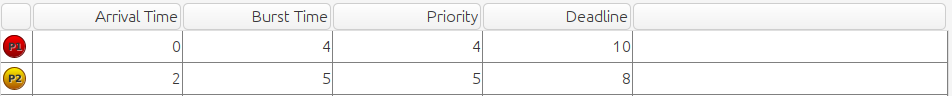
\includegraphics[width=0.8\linewidth]{Assets/Betriebssystem_uebung/u3_a1.png}
\end{center}

%##########################################
\subsection{Aufgabe 2: Round Robin mit Prioritäten}
\textit{Die Scheduling-Strategie Round Robin soll ein möglichst faires Scheduling mehrerer Prozesse ermöglichen. In der Vorlesung haben Sie die zusätzliche Möglichkeit kennengelernt, Round Robin mit einem Prioritätenschema zu kombinieren. Wir wollen uns in dieser Aufgabe auf statische Prioritäten beschränken, auch wenn diese in bestimmten, realen Anwendungen während der Abarbeitung von Prozessen (dynamisch) neu bestimmt werden können.}
\vspace{10mm}
\textit{a) Implementieren Sie Round Robin mit Prioritäten. Sie finden dazu bereits eine Implementierung der Strategie ohne Berücksichtigung von Prioritäten unter Simulation → Source Packages → frm.pssav.sim → RoundRobinScheduler.java, die Sie entsprechend anpassen müssen.}
\vspace{10mm}
(siehe Netbeans)

\textit{b) Von welchen Faktoren ist die Länge einer Zeitscheibe in der Praxis abhängig? Von welchen die Priorität? Welcher Unterschied ergibt sich daraus für das Setzen dieser beiden Parameter?}
\vspace{10mm}

\textit{Demonstrieren Sie die Auswirkungen unterschiedlich langer Zeitscheiben sowie unterschiedlicher Prioritäten anhand zweier Szenarien: Eines mit (genügend vielen) sehr kurzen Prozessen, ein anderes mit sehr viel länger rechnenden. Diskutieren Sie, welche realen Einflussfaktoren – die in PSSAV nicht berücksichtigt werden können – hier in der Praxis eine Rolle spielen müssen.}


%##########################################
\subsection{Aufgabe 3: Linux-Scheduling}
\textit{Moderne Universal-Betriebssysteme müssen heute mit Prozessen und Threads sehr unterschiedlichen Charakters umgehen können. Einerseits könnten z. B. Echtzeitprozesse zur Audio/Video-Verarbeitung ablaufen, andererseits gibt es auch zeitunabhängige aber rechenzeitintensive Prozesse wie beispielsweise das in der Vorlesung gezeigte Ray-Tracing-Programm.}
\vspace{10mm}
\textit{a) Recherchieren Sie für das Betriebssystem Linux die für das Scheduling von Prozessen verantwortlichen funktionalen Komponenten (Scheduling-Subsystem) und ermitteln Sie, welche Schedulingstrategien Linux unterstützt.}
\vspace{10mm}
\begin{itemize}
    \item Linux verwendet seit Kernelversion 2.6.23 CFS (Completely Fair Scheduler)
    \item Es gibt verschiedene Schedulingstrategien wie:
          \begin{itemize}
              \item SCHED\_FIFO: First in First out Scheduling
              \item SCHED\_RR: Round-Robin Scheduling
              \item SCHED\_DEADLINE: Sporadic task model deadline scheduling
              \item SCHED\_OTHER: Default Linux time-sharing scheduling
              \item SCHED\_BATCH: Scheduling batch processes
              \item SCHED\_IDLE: Scheduling very low priority jobs
          \end{itemize}
    \item Der Scheduler selbst ist eine Kernelkomponente welche entscheidet, welcher ausführbare Thread als nächster auf der CPU ausgeführt werden wird. Die von Linux verwendete Schedulingklasse basiert auf der POSIX Expansion für Echtzeitcomputersysteme.
\end{itemize}

\textit{Damit das Betriebssystem sinnvoll mit diesen unterschiedlichen Prozessen umgehen kann, müssen Prozesse selbst ihre Lastmerkmale dem Betriebssystem mitteilen (neben der Beobachtung und Klassifizierung der Prozesse durch das Betriebssystem selbst). Eine sehr einfache Möglichkeit, das Scheduling von Prozessen zu beeinflussen, besteht in der Vergabe unterschiedlicher (Basis-)Prioritäten, auf deren Grundlage die dynamische Änderung durch das Betriebssystem vorgenommen wird. Für jeden regulären Prozess steht hierzu der Systemaufruf $nice$ zur Verfügung; ein Nutzer kann die Priorität seiner Prozesse mithilfe der Ausführung
    der Kommandos $nice$ oder $renice$ verschlechtern (der Name deshalb, weil er damit "nett" zu anderen Prozessen ist).}
\vspace{10mm}
\textit{b) Starten Sie zwei gleichartige rechenzeitintensive Prozesse (ggf. hierfür ein einfaches Programm schreiben), die lange genug rechnen. Demonstrieren und erläutern Sie deren Verhalten, wenn einerseits beide die gleiche Priorität haben und andererseits ein Prozess seine Priorität verringert hat. Überlegen Sie sich geeignete Demonstrationsmöglichkeiten.}
\vspace{10mm}

\begin{itemize}
	\item Verwendete taskset 0x1 ./simpleproc um die selben Prozessorcores zu verwenden
	\item über top fand ich die Prozessorauslastung in Prozent heraus
	\item Darüber hinaus zeigte sich bei meinen Programmen mit verschiedenen Prioritäten allerdiungs nicht wirklich ein Unterschied. Einzig für Prozess wie den NTP Deamon oder ASLA/Pulseaudio würde es Sinn machen, denn wenn man beispielsweise der musikausgebenden Anwendung sehr viel Priorität wegnimmt und beispielsweise einem unbedeutenden Programm hinzufügen würde, so würde man hören, dass die Musik lückenhaft wird, bzw. das Programm unresponsiv wird. 
\end{itemize}
Siehe auch Linux Manpages

\textit{
    Hinweise:
    Falls Sie nicht selbst geeignete Ideen haben: Beispielsweise lassen sich lange laufende Prozesse durch Hochzählen einer Variablen vom Typ long int (lange ganzzahlige Variable) erzeugen, oder durch Starten mehrerer Instanzen einer ausreichend anspruchsvollen Anwendung Ihrer Wahl (anspruchsvoll für den Hauptprozessor, nicht nur für die Grafikhardware).\\
    Falls Sie an einem System mit einem Mehrkernprozessor arbeiten, könnten die zu zeigenden Effekte unsichtbar bleiben, wenn z. B. jeder Prozess auf einem eigenen Prozessorkern läuft. Beschäftigen Sie sich hierzu z. B. mit dem Systemaufruf $sched_setaffinity()$.
}
\vspace{10mm}


\newpage
%%%%%%%%%%%%%%%%%%%%%%%%%%%%%%%%%%%%%%%%%%%%%%%%%%%%%%%%%%%%%%%%%%%%%%%%%%%%%%%%%%%%%%%%%%%%%%%%%%%%%%%%%%%%%%%%%%%%
\section{Übung 4}
%##########################################
\subsection{Repetitorium}
\begin{description*}
    \item[Welche prinzipiellen Probleme entstehen, wenn parallel ablaufende Threads auf einen gemeinsamen Speicherbereich zugreifen? Welche beiden konkreten Synchronisationsprobleme bestehen beim Erzeuger/Verbraucher-Problem?]
    \item[In der Vorlesung haben wir binäre Semaphore kennen gelernt, die innerhalb eines kritischen Abschnitts strengen wechselseitigen Ausschluss garantieren. Eine allgemeinere Form der Semaphore lässt eine gewisse feste Anzahl von Aktivitäten in einen kritischen Abschnitt hinein, bevor die Sperrwirkung eintritt. Wie können derartige Semaphore implementiert werden?]
    \item[Wie viele Semaphore braucht man mindestens zur Lösung des allgemeinen Erzeuger/Verbraucher-Problems?]
    \item[Wir haben Bedingungsvariable im Kontext Hoare’scher Monitore kennen gelernt. Ist ein derartiges Synchronisationsmodell (Warten auf Erfüllung einer Bedingung) nicht auch außerhalb und losgelöst vom Monitormodell nützlich? Falls ja, worauf müsste man in einem solchen Fall achten?]
\end{description*}
%##########################################
\subsection{Aufgabe 1: Das Problem des schlafenden Barbiers}
\textit{In einem Friseurladen gibt es einen Friseur, einen Frisierstuhl (an dem der Friseur arbeitet) und n Stühle für wartende Kunden. Entwickeln Sie einen Algorithmus, der unter den nachfolgenden Annahmen Friseur und Kunden so synchronisiert, dass jeder wartende Kunde (irgendwann) bedient wird.}
\begin{itemize*}
    \item Der Friseur und alle Kunden agieren parallel.
    \item Falls keine Kunden da sind, geht der Friseur schlafen.
    \item Wenn ein Kunde kommt, während der Friseur schläft, weckt der Kunde den Friseur und setzt sich in den Frisierstuhl (und wird bedient).
    \item Wenn ein Kunde eintrifft, während der Friseur arbeitet und ein freier Kundenstuhl vorhanden ist, setzt sich der Kunde und wartet.
    \item Trifft ein Kunde ein, während der Friseur arbeitet und alle Kundenstühle belegt sind, verlässt der Kunde den Friseurladen sofort wieder.
    \item Wenn der Friseur mit dem Bedienen eines Kunden fertig ist, verlässt dieser Kunde den Friseurladen und einer der wartenden Kunden (falls vorhanden) belegt den Frisierstuhl und wird bedient (sonst gilt Bedingung 2).
\end{itemize*}
\vspace{10mm}


%##########################################
\subsection{Aufgabe 2: Das Achterbahnproblem}
\textit{Das Achterbahnproblem nach J.S. Herman wird durch das folgende Szenario beschrieben. Eine Anzahl $n$ von "Vergnügungssüchtigen" (im Folgenden Passagiere genannt) versucht, möglichst oft eine Fahrt mit einem der $m$ zur Verfügung stehenden Achterbahnwagen zu unternehmen. Dabei gelten allerdings die folgenden Bedingungen.
    \begin{itemize*}
        \item Ein Wagen darf nur losfahren, wenn er voll besetzt ist. (Dabei gilt: Jeder Wagen fasst $c$ Passagiere, wobei die Gesamtzahl der beteiligten Passagiere mehr als nur einen Wagen füllt, d. h. $c < n$.)
        \item Wenn ein Wagen vollständig besetzt ist, fährt er los.
        \item Wenn der Wagen nach Abschluss der Fahrt wieder anhält, steigen alle Passagiere aus und bemühen sich erneut, in einem "neuen" Wagen eine weitere Fahrt zu unternehmen. (Unter entsprechenden Umständen kann es natürlich auch wieder der gleiche Wagen sein.)
        \item Wagen dürfen sich nicht überholen (was ja beim gegebenen Achterbahnproblem auch technisch nicht möglich ist), d. h. die Reihenfolge der Wagen bleibt immer gleich.
    \end{itemize*}
    Passagiere und Wagen sollen durch Aktivitäten simuliert werden, die synchronisiert werden müssen. Für eine der möglichen Lösungen könnten die folgenden Hinweise hilfreich sein: Bei der Ankunft eines Wagens sollte dieser eine Prozedur $Einsteigen()$ aufrufen, danach sollten $c$ Passagiere ihrerseits eine Prozedur $In_Wagen_Einsteigen()$ aufrufen. Nach beendeter Fahrt sollte ein anhaltender Wagen eine Prozedur $Aussteigen()$ aufrufen, und die sich im Wagen befindenden $c$ Passagiere sollten daraufhin eine Prozedur $Wagen_Verlassen()$ aufrufen.
}
\vspace{10mm}

%##########################################
\subsection{Aufgabe 3: Der Kaffeeautomat}
\textit{Ein Kaffeeautomat, seine Kunden und ein Lieferant, der den Automaten regelmäßig mit Kaffee und Kaffeebechern auffüllt, sollen sich mittels Semaphoren synchronisieren. Synchronisieren Sie das Verhalten dieser Aktivitäten so, dass folgendes Verhalten realisiert wird.
    \begin{itemize*}
        \item Der Automat kann entweder einen Kunden bedienen oder durch den Lieferanten nachgefüllt   werden. Beide Vorgänge sind nicht gleichzeitig möglich!
        \item Ein Kunde muss nach Aufforderung durch den Automaten eine 1-Euro-Münze als Bezahlung einwerfen, erst danach bekommt er seinen Kaffee. (Um eine ungeeignete Betriebsweise auszuschließen, soll angenommen werden, dass sich nur Kunden anmelden, die eine 1-Euro-Münze parat haben – und nach Aufforderung natürlich auch einwerfen!)
        \item Der Lieferant bekommt durch den Automaten mitgeteilt, dass dieser für den Auffüllvorgang bereit ist.
        \item Ein einmal gestarteter Vorgang (Bedienen bzw. Auffüllen) kann nicht mehr unterbrochen werden. Eine neue Anmeldung (durch den nächsten Kunden oder den Lieferanten) wird erst nach Abschluss dieses Vorgangs akzeptiert.
        \item Der nächste Kunde und der Lieferant können sich jeweils unabhängig voneinander beim Automaten anmelden. Die Reihenfolge der Bedienung hängt dann davon ab, in welcher Reihenfolge die Anmeldungen erfolgen.
        \item Lieferant und Kunde bekommen den Abschluss des jeweiligen Vorgangs durch den Automaten mitgeteilt.
        \item Falls der Kaffeevorrat verbraucht ist oder keine Becher mehr vorhanden sind, versetzt sich der Automat selbst in einen Wartezustand und wartet bis er durch den Lieferanten wieder befüllt ist.
    \end{itemize*}
}
\vspace{10mm}


\newpage
%%%%%%%%%%%%%%%%%%%%%%%%%%%%%%%%%%%%%%%%%%%%%%%%%%%%%%%%%%%%%%%%%%%%%%%%%%%%%%%%%%%%%%%%%%%%%%%%%%%%%%%%%%%%%%%%%%%%
\section{Übung 5}
%##########################################
\subsection{Diskussionsfragen}
\paragraph{Frage 1: Speicherbasierte vs. nachrichtenbasierte Interprozesskommunikation}
\textit{Stellen Sie sich vor, Ihre Übungsgruppe müsste ein Videoschnittsystem entwickeln, welches aus Robustheitsgründen die Berechnung komplexer Effekte, die En- und Dekodierung verschiedener Formate sowie die Steuerung der gesamten Applikation in jeweils unterschiedlichen Prozessen implementieren soll. Diese Prozesse müssen natürlich miteinander kommunizieren und dabei neben Kontrollinformationen auch die zu verarbeitenden Video- und Audiodaten austauschen.
    Prinzipiell stehen dafür nachrichtenbasierte und speicherbasierte Kommunikationsmechanismen zur Verfügung. Für welche der existierenden Mechanismen würden sie sich entscheiden, um einerseits Kontrollinformationen und andererseits Mediendatenströme auszutauschen? Begründen Sie Ihre Antwort.\\
    Hinweis: Klären Sie zuerst, was die prinzipiellen Vor- und Nachteile dieser beiden Kommunikationsvarianten sind. Betrachten Sie anschließend die Kommunikationsmuster und Anforderungen der beiden Klassen (Kontroll- und Multimediadaten), bevor Sie eine Empfehlung geben.
}

\vspace{10mm}
\paragraph{Frage 2: Synchronisation durch Semaphore}
\textit{Bei asynchroner nachrichtenbasierter Kommunikation kommen stets Warteschlangen zum Einsatz, um unterschiedliche Geschwindigkeiten der Sender- und Empfängerprozesse auszugleichen. Der Zugriff auf diese Warteschlangen muss aus verschiedenen Gründen durch Synchronisationsmechanismen (z. B. Semaphore) geregelt werden. Was sind diese Gründe und weshalb sind insgesamt drei Semaphore pro Warteschlange notwendig?}

\vspace{10mm}
\paragraph{Frage 3: Synchronisationsvarianten bei nachrichtenbasierter Kommunikation}
\textit{Welche Nachteile asynchroner Kommunikation treten beim Einsatz synchroner Varianten der Sende- und Empfangsoperationen nicht auf? Warum ist es trotzdem manchmal sinnvoll oder unumgänglich, die asynchronen Varianten einzusetzen? Nennen Sie mindestens drei Beispiele realer Applikationen, in denen asynchron kommuniziert wird.}

\vspace{10mm}
\paragraph{Frage 4: Management asynchroner Ereignisse}
\textit{Welche Alternativen haben die Entwickler von Betriebssystemen, um mit asynchron auftretenden
    Ereignissen (Mausbewegungen, Einstecken von USB-Geräten etc.) umzugehen? Welche Technik
    erlaubt es auch einem Benutzerprozess, auf asynchrone Ereignisse zu reagieren, ohne direkten
    Hardwarezugriff zu haben?}

%##########################################
\subsection{Aufgabe 1: Nachrichtenwarteschlangen (Message Queues)}
\textit{a) Recherchieren Sie die Funktionsweise, Charakteristiken und Eigenschaften von Message Queues. Wie wird der Kontrollfluss der Prozesse dabei durch das Betriebssystem gesteuert (z. B. Synchronisation durch Blockierungen, durch die Ankunft von Daten usw.)?}
\vspace{10mm}

\textit{b) In der Anlage zu dieser Übungsaufgabe (u4-a1-anlage) befinden sich ein Server- und ein Client-Programm, die beide Lücken enthalten. Vervollständigen und übersetzen Sie die Programme. Starten Sie anschließend zuerst den Server und dann den Client. Falls Sie die Lücken richtig ausgefüllt haben, muss das Client-Programm ein "Passwort" an den Server senden und anschließend ein Geheimnis ausgeben, das es vom Server als Antwort erhalten hat.}
\vspace{10mm}

%##########################################
\subsection{Aufgabe 2: Gemeinsamer Speicher (Shared Memory)}
\textit{a) Recherchieren Sie die Funktionsweise, Charakteristiken und Eigenschaften von Shared Memory. Wie wird der Kontrollfluss der Prozesse dabei durch das Betriebssystem gesteuert? (Wann und wodurch erfolgt eine Synchronisation?)}
\vspace{10mm}

\textit{b) In der Anlage zu dieser Übungsaufgabe (u4-a2-anlage) befinden sich ein Server- und ein Client-Programm, die beide Lücken enthalten. Vervollständigen und übersetzen Sie die Programme. Starten Sie anschließend zuerst den Server und dann den Client. Falls Sie die Lücken richtig ausgefüllt haben, muss das Client-Programm ein "Passwort" an den Server senden und anschließend ein Geheimnis ausgeben, das es vom Server als Antwort erhalten hat.\\
    Hinweis: An den verwendeten Semaphoroperationen sind keine Änderungen notwendig.}
\vspace{10mm}

%##########################################
\subsection{Aufgabe 3: Benannte Pipes (Named Pipes, FIFOs)}
\textit{a) Recherchieren Sie die Funktionsweise, Charakteristiken und Eigenschaften von Pipes und Named Pipes. Wie wird der Kontrollfluss der Prozesse dabei durch das Betriebssystem gesteuert? (Wann und wodurch erfolgt eine Synchronisation?)}
\vspace{10mm}


\textit{b) In der Anlage zu dieser Übungsaufgabe (u4-a3-anlage) befinden sich ein Server- und ein Client-Programm, die beide Lücken enthalten. Vervollständigen und übersetzen Sie die Programme. Starten Sie anschließend zuerst den Server und dann den Client. Falls Sie die Lücken richtig ausgefüllt haben, muss das Client-Programm ein "Passwort" an den Server senden und anschließend ein Geheimnis ausgeben, das es vom Server als Antwort erhalten hat.}
\vspace{10mm}


\newpage
%%%%%%%%%%%%%%%%%%%%%%%%%%%%%%%%%%%%%%%%%%%%%%%%%%%%%%%%%%%%%%%%%%%%%%%%%%%%%%%%%%%%%%%%%%%%%%%%%%%%%%%%%%%%%%%%%%%%
\section{Übung 6}
%##########################################
\subsection{Repetitorium}
\begin{description*}
    \item[Wodurch sind die Mehrkosten eines Systemaufrufs im Vergleich zu einem regulären Prozeduraufruf bedingt?]
    \item[Für die Behandlung asynchroner Unterbrechungen (Interrupts) gibt es mehrere Modelle, u.a. auch das Modell des erzwungenen Prozeduraufrufs und das Pop-up-Thread-Modell. Worin bestehen die Unterschiede bei diesen beiden Modellen?]
    \item[Vor welchem fehlerhaften Verhalten von Anwendungsprozessen schützen private virtuelle Adressräume? Auf welche Weise üben Adressräume ihre Schutzfunktion aus? Aus welchen Gründen kann es sinnvoll sein, zwei oder mehreren Prozessen gleichzeitig Zugriff auf einen gemeinsamen Speicherbereich zu geben?]
    \item[Warum ist es nur schwer möglich, schon während der Übersetzung eines Programms dafür zu sorgen, dass es bei der Ausführung keine Speicherzugriffssünden begeht?]
    \item[Warum ist eine optimale Pagingstrategie im Allgemeinen nicht erreichbar? Unter welcher speziellen Voraussetzung geht dies dennoch?]
    \item[Wie viele Seitentabellen gibt es in einem anlaufenden Betriebssystem mit virtueller Speicherverwaltung? Benötigt ein E/A-Adressraum eine eigene Seitentabelle?]
    \item[Was ist die Arbeitsmenge (Working Set) eines Prozesses? Wozu dient sie? Zu welchen Zeitpunkten bzw. unter welchen Voraussetzungen stimmt sie mit der Menge der für einen Prozess eingelagerten Seiten (Resident Set) überein?]
    \item[Welche Aufgaben hat eine MMU? Wozu dient ein TLB (Translation Look-aside Buffer)? Wann wird er von wem wozu benutzt?]
    \item[Seitentabellen können je nach Adressraumgröße sehr groß werden. Mit diesem Problem gehen mehrstufige Seitentabellen um. Gegeben sei die Aufteilung einer virtuellen 32-Bit-Adresse für ein zweistufiges Abbildungsverfahren (P i als Seitentabellenindex i. Stufe).]
    \begin{itemize*}
        \item Wie groß ist die Seitentabelle? Wie groß ist die Seitenrahmen- bzw. Kachelgröße?
        \item Um welchen Faktor reduziert sich die Größe der Seitentabelle, die ständig im Hauptspeicher zu halten ist, bei einem zweistufigen Seitentabellenverfahren gegenüber einer einstufigen Seitentabelle?
        \item Welche Größe haben die Seitentabellen bei einstufigen bzw. zweistufigen Verfahren bei einer Eintragsbreite von jeweils 4 Byte?
    \end{itemize*}
    \item[Bei einer Seitengröße von 8 KiByte und einem virtuellen Adressraum der Größe $2^{64}$: Wie groß wäre eine einstufige, nicht invertierte Seitentabelle eines Prozesses, wenn jeder Seiteneintrag in der Tabelle 32 Bit (= $2^2$ Byte) groß ist?]
\end{description*}
%##########################################
\subsection{Aufgabe 1: Systemaufrufe}
\textit{Dienstleistungen des Betriebssystems (z. B. Erzeugen von Prozessen, Threads oder Dateien) werden unter Zwischenschaltung von Stellvertreterprozeduren aufgerufen (z. B. für Programme in der Sprache C finden diese sich bei Linux-Systemen meist in der C-Standardbibliothek libc), die dann über einen aufwändigeren als den Prozedurmechanismus den tatsächlichen Sprung ins Betriebssystem implementieren.}
\vspace{10mm}
\textit{a) Warum kann man aus einem Anwendungsprogramm nicht direkt eine im Betriebssystem implementierte Prozedur aufrufen? Erläutern Sie die gängige alternative Verfahrensweise. Welche prinzipiellen Bestandteile enthalten die genannten Stellvertreterprozeduren?}
\vspace{10mm}


\textit{b) In der Anlage zur Aufgabe finden Sie das Programm $syscall.c;$ dort ist beispielhaft ein Systemaufruf manuell implementiert. Warum enthält das Unterprogramm Assemblerbefehle? Erweitern Sie nach obigem Muster Ihren "eigenen" $exit()$-Systemaufruf $my\_exit()$, indem Sie das begonnene Fragment ergänzen. Demonstrieren Sie dessen korrekte Funktionsweise.\\
    Hinweis: Mit dem Systemaufruf $wait()$ kann man den Terminierungsstatus von Kindprozessen überprüfen. Um das Programm zu kompilieren, auszuführen und seinen Rückgabewert anzuzeigen, können Sie alternativ das beigefügte Shell-Skript $run.sh$ benutzen.
}
\vspace{10mm}

\textit{c) Vor der Einführung des Maschinenbefehls $syscall$ in modernen 64-Bit-Architekturen musste zum Auslösen eines Systemaufrufs durch ein Anwendungsprogramm ein spezieller Interrupt (trap) ausgelöst werden. Recherchieren Sie, welche Vorteile die Verwendung von $syscall$ gegenüber dieser konventionellen Verfahrensweise hat. Auch heute noch wird aus Gründen der Abwärtskompatibilität und zur Unterstützung spezieller Prozessorarchitekturen der $trap$-Mechanismus durch den Linux-Kernel unterstützt. Schaffen Sie es, Ihre $my\_exit()$-Implementierung mittels Ersetzen der $syscall$ Instruktion durch einen Trap-Interrupt ($int \$ 0x80$) entsprechend zu portieren?\\
    Beachten Sie, dass dabei Systemaufruf-Nummern für 32-Bit-Hardwarearchitekturen und andere Register zu verwenden sind.
}
\vspace{10mm}


\textit{Tipp zur gesamten Aufgabenstellung: Unter Linux können Sie mit $strace <Programm>$ u.a. die Systemaufrufe eines Programms verfolgen.}
\vspace{10mm}


%##########################################
\subsection{Aufgabe 2: Ereignismanagement mit Linux-Signalen}
\textit{In Linux-Systemen kann mittels des Signalmechanismus eine Behandlung bestimmter Ereignisse auf Prozessebene stattfinden (aus der Vorlesung als "Interruptbehandlung auf Prozessebene" bekannt).\\
    Dieses Prinzip soll nun mit mittels sogenannter Dämon-Prozesse (daemons) veranschaulicht werden. Dabei handelt es sich um Hintergrundprozesse, die i. d. R. im Verlauf des Boot-Vorgangs gestartet werden und keine direkte Benutzerinteraktion vorsehen.
    So kümmert sich beispielsweise der Line Printer Daemon (lpd) oder der Common Unix Printing System Daemon (cupsd) darum, Druckaufträge nebenläufig zu anderen Benutzerprozessen abzuwickeln.
    Eine typische Verwendung von Signalen ist beispielsweise, einem Dämon die Änderung seiner Konfigurationsdatei(en) zur Laufzeit mitzuteilen, woraufhin diese erneut eingelesen werden sollen.
    Hierfür hat sich die Benutzung des Signals $SIGHUP$ etabliert.
}
\vspace{10mm}

\textit{a) Recherchieren Sie, welche Signale der für Unix-Systeme etablierte POSIX-Standard vorsieht und wie diese einem Prozess zugestellt werden. Demonstrieren Sie in der Übung, wie man auf der Kommandozeile einem beliebigen Prozess ein Signal (z. B. SIGHUP oder SIGKILL) senden kann.
    Informationen hierzu finden Sie wie immer in den Linux-Manpages oder im Handbuch zur C-Standardbibliothek libc.}
\vspace{10mm}

\textit{In der Anlage zu dieser Aufgabe stellen wir Ihnen den Quellcode eines kleinen Dämon-Prozesses zur Verfügung. Zur besseren Demonstration haben wir darauf verzichtet, ihn als Hintergrundprozess zu initialisieren; er läuft daher wie ein Nutzerprozess und kann so seine Ausgaben auf der Kommandozeile sichtbar machen.}
\vspace{10mm}

\textit{b) Starten Sie den mitgelieferten Dämon und demonstrieren Sie, wie dieser auf verschiedene Signale reagiert. Erklären Sie das Verhalten mithilfe Ihrer Recherche aus Teilaufgabe a).}
\vspace{10mm}

\textit{c) Erweitern Sie den Dämon nun um die Fähigkeit, seine Konfigurationsdateien neu zu laden, wann immer er das Signal SIGHUP empfängt. Sie können dazu als Reaktion auf das Signal die bereits vorhandene Funktion $load_config()$ aufrufen.}
\vspace{10mm}

\textit{d) Schaffen Sie es, durch Reaktion auf die Signale SIGTERM und SIGKILL ein explizites Terminieren des Prozesses durch den Benutzer zu verhindern? Demonstrieren und erklären Sie Ihre Ergebnisse.}
\vspace{10mm}


%##########################################
\subsection{Aufgabe 3: Virtuelle Speicherverwaltung von Linux-Systemen}
\textit{Stellen Sie das virtuelle Speichermanagement von Linux-Systemen vor. Gehen Sie dabei insbesondere auf die Struktur der Seitentabellen und die Seitengröße ein.
    Virtuelle Speicherverwaltung bietet auch eine elegante Möglichkeit zur dynamischen Speicherverwaltung, d. h. je nach Bedarf den von einem Prozess belegten Speicherplatz zu vergrößern bzw. wieder zu verkleinern.
    Die Motivation zur Integration dieser Technik in den Linux-Kernel war die Einführung dynamischer Objekte in Programmiersprachen, die z. B. mittels new() während des Programmablaufs bei Bedarf neue Variablen, insbesondere große Arrays, erzeugen und auch wieder löschen können. Zum Ansprechen der entsprechenden Implementierungen in Linux, werden auf Nutzerebene die Funktionen malloc() ("memory allocation") und free() (Wiederfreigeben von Speicher) bereitgestellt. Beide Funktionen sind über Eintrittspunkte in die C-Standard-Bibliothek implementiert. Freier Speicher wird dabei vom Heap besorgt.}
\vspace{10mm}

\textit{a) Erklären Sie diesen Begriff im Linux-Kontext. Stellen Sie dann die beiden obigen Funktionen vor und demonstrieren Sie ihre Benutzung.}
\vspace{10mm}

\textit{Im Linux-Kern benutzen $malloc()$ und $free()$ den Systemaufruf $brk()$ ("break"), der ebenso freien Speicher requiriert, aber für die Verwendung als Programmierschnittstelle nicht empfohlen wird. Dieser ändert den so genannten Programm-"break".}
\vspace{10mm}
\textit{b) Was bedeutet dies? Wie kann man dessen aktuellen Wert sowie dessen Maximalwert feststellen?}
\vspace{10mm}

\textit{c) Wodurch unterscheiden sich die Funktionen $malloc()/free()$ und $brk()$?}
\vspace{10mm}


\end{document}